
\centering
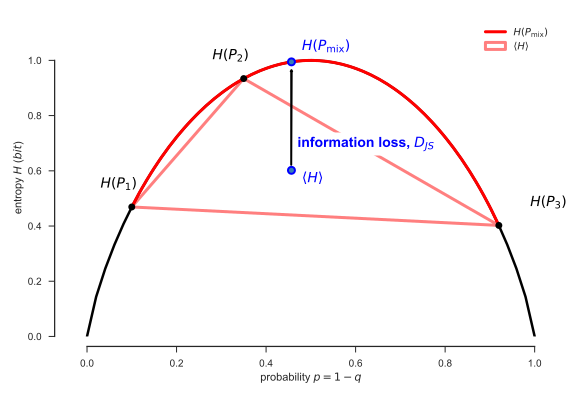
\includegraphics[width=1\textwidth]{jsd_entropy.svg}
\caption{
    Jensen-Shannon Divergence (JSD) in terms of Shannon entropy.
    The black curve shows the entropy function of a binary PDF in terms of $p=1-q$ and black dots designate three example PDFs (black).
    The locations of the corresponding quantities for calculating JSD depend on the weights but can only lie on the red curve segment and polygon , respectively.
    Blue dots show an example mixture and the corresponding informationn loss.
    }
\label{fig:jsd_entropy}

